\documentclass{beamer}
%
% Choose how your presentation looks.
%
% For more themes, color themes and font themes, see:
% http://deic.uab.es/~iblanes/beamer_gallery/index_by_theme.html
%
\mode<presentation>
{
  \usetheme{default}      % or try Darmstadt, Madrid, Warsaw, ...
  \usecolortheme{default} % or try albatross, beaver, crane, ...
  \usefonttheme{default}  % or try serif, structurebold, ...
  \setbeamertemplate{navigation symbols}{}
  \setbeamertemplate{caption}[numbered]
  \setbeamertemplate{footline}[frame number]
  \setbeamertemplate{itemize items}[circle]
  \setbeamertemplate{theorems}[numbered]
  \setbeamercolor*{structure}{bg=white,fg=blue}
  \setbeamerfont{block title}{size=\normalsize}
  \setbeamercolor{bibliography entry author}{fg=black}
  \setbeamercolor{bibliography entry title}{fg=black}
  \setbeamercolor{bibliography entry note}{fg=black}
}

% \newtheorem{proposition}[theorem]{Proposition}
% \theoremstyle{definition}
% \newtheorem{algorithm}[theorem]{Algorithm}
% \newtheorem{idea}[theorem]{Idea}

\usepackage[english]{babel}
\usepackage[utf8]{inputenc}
\usepackage[T1]{fontenc}
% \usepackage{aligned-overset}
\usepackage{alltt}
\usepackage{amsmath}
\usepackage{csquotes}
% \usepackage{multicol}
% \usepackage{stmaryrd}
\usepackage{tabularx}
\usepackage{tikz}
\usetikzlibrary{patterns}
\usetikzlibrary{intersections}
\usepackage{pgfplots}
\usepgfplotslibrary{fillbetween}
\usepgfplotslibrary{dateplot}
\usepackage{pgfplotstable}
% \usepackage{booktabs}
\usepackage[final]{microtype}
\usepackage{caption}
\usepackage{amsmath}
\usepackage{mathtools}
\usepackage{amsthm,thmtools}
% \usepackage[nottoc]{tocbibind}
% \usepackage[ruled]{algorithm2e}
\usepackage{enumerate}
\usepackage{tabularx}
\usepackage[italic]{esdiff}
\usepackage{subcaption}
\usepackage{ltablex}
\usepackage{multirow}

% Settings for pgfplots
\pgfplotsset{compat=newest}

% \renewcommand\tabularxcolumn[1]{m{#1}}
% \newcolumntype{R}{>{\raggedleft\arraybackslash}X}=

\def\code#1{\texttt{\frenchspacing#1}}
\def\padding{\vspace{0.5cm}}
\def\spadding{\vspace{0.25cm}}
\def\b{\textcolor{blue}}
\def\r{\textcolor{red}}
\def\g#1{{\usebeamercolor[fg]{block title example}{#1}}}

% % fix for \pause in align
% \makeatletter
% \let\save@measuring@true\measuring@true
% \def\measuring@true{%
%   \save@measuring@true
%   \def\beamer@sortzero##1{\beamer@ifnextcharospec{\beamer@sortzeroread{##1}}{}}%
%   \def\beamer@sortzeroread##1<##2>{}%
%   \def\beamer@finalnospec{}%
% }
% \makeatother

\DeclarePairedDelimiter{\norm}{\lVert}{\rVert}

\usepackage[sorting=ynt,style=alphabetic]{biblatex}
\addbibresource{sources.bib}

\renewcommand{\footnotesize}{\tiny}

\begin{document}

\title[Implementation of Algorithms for Right-Sizing Data Centers]{Implementation of Algorithms for \\ Right-Sizing Data Centers}
\institute{Department of Informatics \\ Technical University of Munich}
\author{\begin{tabular}{r@{ }l}
Author:      & Jonas Hübotter \\[1ex]
Supervisor:  & Prof. Dr. Susanne Albers\\
Advisor:     & Jens Quedenfeld\\
\end{tabular}}
\date{August 13, 2021}

\begin{frame}
  \titlepage
\end{frame}

\begin{frame}{Outline}
 \tableofcontents[subsectionstyle=hide, subsubsectionstyle=hide]
\end{frame}
% \AtBeginSection[]
%   {
%      \begin{frame}[allowframebreaks]{Plan}
%      \tableofcontents[currentsection, sectionstyle=show/hide, hideothersubsections]
%      \end{frame}
%   }

\section{Motivation}

\begin{frame}{Motivation}
    \begin{itemize}
        \item data centers use between 1\% and 3\% of global energy \footfullcite{Shehabi2016}, which is estimated to increase\footfullcite{Jones2018}\pause
        \item most data centers are statically provisioned, leading to average utilization levels between 12\% and 18\%\footfullcite{Whitney2014}\pause
        \item typically servers operate at energy efficiency levels between 20\% and 30\%\footfullcite{Barroso2007}\pause
        \item when idling, servers consume half of their peak power\footnotemark[\value{footnote}]
    \end{itemize}
\end{frame}

\section{Problem}

\begin{frame}{Problem}
\centering
\tikzset{every picture/.style={line width=0.75pt}} %set default line width to 0.75pt

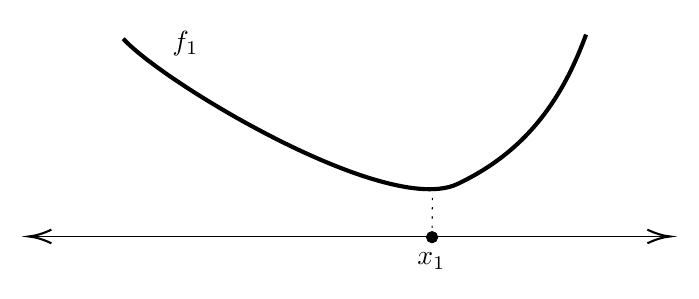
\begin{tikzpicture}[x=0.75pt,y=0.75pt,yscale=-1,xscale=1]
%uncomment if require: \path (0,308); %set diagram left start at 0, and has height of 308

%Straight Lines [id:da3912851178909138]
\draw    (331,135.33) -- (636,135.33) ;
\draw [shift={(638,135.33)}, rotate = 180] [color={rgb, 255:red, 0; green, 0; blue, 0 }  ][line width=0.75]    (10.93,-3.29) .. controls (6.95,-1.4) and (3.31,-0.3) .. (0,0) .. controls (3.31,0.3) and (6.95,1.4) .. (10.93,3.29)   ;
\draw [shift={(329,135.33)}, rotate = 0] [color={rgb, 255:red, 0; green, 0; blue, 0 }  ][line width=0.75]    (10.93,-3.29) .. controls (6.95,-1.4) and (3.31,-0.3) .. (0,0) .. controls (3.31,0.3) and (6.95,1.4) .. (10.93,3.29)   ;
\only<2>{
%Shape: Circle [id:dp9366405058886342]
\draw  [fill={rgb, 255:red, 0; green, 0; blue, 0 }  ,fill opacity=1 ] (520.67,135.67) .. controls (520.67,134.19) and (521.86,133) .. (523.33,133) .. controls (524.81,133) and (526,134.19) .. (526,135.67) .. controls (526,137.14) and (524.81,138.33) .. (523.33,138.33) .. controls (521.86,138.33) and (520.67,137.14) .. (520.67,135.67) -- cycle ;
%Straight Lines [id:da6017657532306151]
\draw  [dash pattern={on 0.84pt off 2.51pt}]  (523.33,135.67) -- (523.52,112.05) ;
% Text Node
\draw (515,142) node [anchor=north west][inner sep=0.75pt]    {$x_{1}$};
}

%Curve Lines [id:da9412769336006994]
\draw [line width=1.5]    (374.52,40.05) .. controls (393.52,61.05) and (501.52,126.05) .. (535.52,110.05) .. controls (569.52,94.05) and (586.52,68.05) .. (597.52,38.05) ;
% Text Node
\draw (397,35) node [anchor=north west][inner sep=0.75pt]    {$f_{1}$};
\end{tikzpicture}
\end{frame}
\begin{frame}{Problem}
\centering
\tikzset{every picture/.style={line width=0.75pt}} %set default line width to 0.75pt

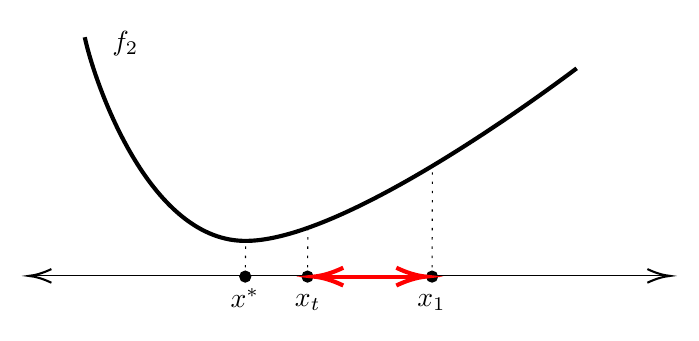
\begin{tikzpicture}[x=0.75pt,y=0.75pt,yscale=-1,xscale=1]
%uncomment if require: \path (0,308); %set diagram left start at 0, and has height of 308

%Straight Lines [id:da8132100594867722]
\draw    (7,136.33) -- (312,136.33) ;
\draw [shift={(314,136.33)}, rotate = 180] [color={rgb, 255:red, 0; green, 0; blue, 0 }  ][line width=0.75]    (10.93,-3.29) .. controls (6.95,-1.4) and (3.31,-0.3) .. (0,0) .. controls (3.31,0.3) and (6.95,1.4) .. (10.93,3.29)   ;
\draw [shift={(5,136.33)}, rotate = 0] [color={rgb, 255:red, 0; green, 0; blue, 0 }  ][line width=0.75]    (10.93,-3.29) .. controls (6.95,-1.4) and (3.31,-0.3) .. (0,0) .. controls (3.31,0.3) and (6.95,1.4) .. (10.93,3.29)   ;
% \only<2>{
% %Shape: Circle [id:dp9366405058886342]
% \draw  [fill={rgb, 255:red, 0; green, 0; blue, 0 }  ,fill opacity=1 ] (520.67,135.67) .. controls (520.67,134.19) and (521.86,133) .. (523.33,133) .. controls (524.81,133) and (526,134.19) .. (526,135.67) .. controls (526,137.14) and (524.81,138.33) .. (523.33,138.33) .. controls (521.86,138.33) and (520.67,137.14) .. (520.67,135.67) -- cycle ;
% %Straight Lines [id:da6017657532306151]
% \draw  [dash pattern={on 0.84pt off 2.51pt}]  (523.33,135.67) -- (523.52,112.05) ;
% % Text Node
% \draw (515,142) node [anchor=north west][inner sep=0.75pt]    {$x_{1}$};
% }

%Curve Lines [id:da37061921880533877]
\draw [line width=1.5]    (32,21.33) .. controls (36.36,41.81) and (61.25,115.72) .. (106,119.33) .. controls (150.75,122.95) and (246.43,53.26) .. (269,36.33) ;
% Text Node
\draw (44,17) node [anchor=north west][inner sep=0.75pt]    {$f_{2}$};

%Straight Lines [id:da23167830177054616]
\draw  [dash pattern={on 0.84pt off 2.51pt}]  (199.33,136.67) -- (199.52,83.05) ;
%Shape: Circle [id:dp9237316574850754]
\draw  [fill={rgb, 255:red, 0; green, 0; blue, 0 }  ,fill opacity=1 ] (196.67,136.67) .. controls (196.67,135.19) and (197.86,134) .. (199.33,134) .. controls (200.81,134) and (202,135.19) .. (202,136.67) .. controls (202,138.14) and (200.81,139.33) .. (199.33,139.33) .. controls (197.86,139.33) and (196.67,138.14) .. (196.67,136.67) -- cycle ;

% Text Node
\draw (191,144) node [anchor=north west][inner sep=0.75pt]    {$x_{1}$};

\onslide<2->{
%Straight Lines [id:da9850850655894281]
\draw  [dash pattern={on 0.84pt off 2.51pt}]  (109.33,136.67) -- (109.52,120.05) ;
%Shape: Circle [id:dp2801837798690885]
\draw  [fill={rgb, 255:red, 0; green, 0; blue, 0 }  ,fill opacity=1 ] (106.67,136.67) .. controls (106.67,135.19) and (107.86,134) .. (109.33,134) .. controls (110.81,134) and (112,135.19) .. (112,136.67) .. controls (112,138.14) and (110.81,139.33) .. (109.33,139.33) .. controls (107.86,139.33) and (106.67,138.14) .. (106.67,136.67) -- cycle ;

% Text Node
\draw (101,141) node [anchor=north west][inner sep=0.75pt]    {$x^{*}$};
}

\onslide<3->{
%Straight Lines [id:da4019047700825191]
\draw  [dash pattern={on 0.84pt off 2.51pt}]  (139.33,136.67) -- (139.52,113.05) ;
%Shape: Circle [id:dp045787056716331875]
\draw  [fill={rgb, 255:red, 0; green, 0; blue, 0 }  ,fill opacity=1 ] (136.67,136.67) .. controls (136.67,135.19) and (137.86,134) .. (139.33,134) .. controls (140.81,134) and (142,135.19) .. (142,136.67) .. controls (142,138.14) and (140.81,139.33) .. (139.33,139.33) .. controls (137.86,139.33) and (136.67,138.14) .. (136.67,136.67) -- cycle ;

% Text Node
\draw (132,144) node [anchor=north west][inner sep=0.75pt]    {$x_{t}$};

%Straight Lines [id:da25275615888238856]
\draw [color={rgb, 255:red, 255; green, 0; blue, 0 }  ,draw opacity=1 ][line width=1.5]    (145.33,136.67) -- (193.33,136.67) ;
\draw [shift={(196.33,136.67)}, rotate = 180] [color={rgb, 255:red, 255; green, 0; blue, 0 }  ,draw opacity=1 ][line width=1.5]    (14.21,-4.28) .. controls (9.04,-1.82) and (4.3,-0.39) .. (0,0) .. controls (4.3,0.39) and (9.04,1.82) .. (14.21,4.28)   ;
\draw [shift={(142.33,136.67)}, rotate = 0] [color={rgb, 255:red, 255; green, 0; blue, 0 }  ,draw opacity=1 ][line width=1.5]    (14.21,-4.28) .. controls (9.04,-1.82) and (4.3,-0.39) .. (0,0) .. controls (4.3,0.39) and (9.04,1.82) .. (14.21,4.28)   ;
}
\end{tikzpicture}
\end{frame}
\begin{frame}{Problem}
\b{Smoothed online convex optimization} (or \emph{convex function chasing})\footfullcite{Lin2011}:\pause\ Given a convex decision space $\mathcal{X} \subset \mathbb{R}^d$, a norm $\norm{\cdot}$ on $\mathbb{R}^d$, and a sequence $F$ of non-negative convex functions $f_t : \mathcal{X} \to \mathbb{R}_{\geq 0}$\pause, find $x \in \mathcal{X}^T$ such that \begin{align*}
    \sum_{t=1}^T f_t(x_t) + \norm{x_t - x_{t-1}}
\end{align*} is minimized where $T$ is the time horizon and $x_0 = \mathbf{0}$.
\end{frame}
\begin{frame}{Problem}
\begin{itemize}
    \item similar to \emph{online convex optimization} with movement costs and lookahead 1\pause
    \item equivalent to \emph{convex body chasing} in $d + 1$\pause
    \item fundamental incompatibility between competitive ratio and regret even for linear hitting costs in one dimension
\end{itemize}
\end{frame}

\section{Model}

\begin{frame}{Model}
What is the cost of operating a data center with $x_t \in \mathbb{N}_0$ active servers and under load $\lambda_t \in \mathbb{N}_0$?\pause
\begin{itemize}
    \item How to distribute jobs across the active servers?\pause\par
        Distribute evenly across all servers of the same type\footfullcite{Albers2021_2}.
    \item What is the cost associated with such an assignment?\pause\par
        Consisting of energy costs and the revenue loss incurred by a delayed processing of jobs.\pause\par
        Algorithms need to \emph{balance} energy costs and revenue loss.
\end{itemize}\pause\spadding

Movement costs are on the order of operating an idling server for 1-4 hours\footfullcite{Lin2011}.
\end{frame}

\section{Algorithms}

\begin{frame}{Algorithms for one dimension}
\scriptsize
\begin{tabularx}{\textwidth}{r|X|p{2cm}|l}
    problem & algorithm & results & time complexity \\\hline
    \multirow{4}*{fractional} & \onslide<2->{Lazy Capacity Provisioning\footfullcite{Lin2011}} & \onslide<2->{3-competitive} & \onslide<2->{$\mathcal{O}(\tau O_{\epsilon}^{\tau})$} \\
    & \onslide<3->{Memoryless\footfullcite{Bansal2015}} & \onslide<3->{3-competitive} & \onslide<3->{$\mathcal{O}(O_{\epsilon}^1)$} \\
    & \onslide<4->{Probabilistic\footnotemark[\value{footnote}]} & \onslide<4->{2-competitive} & \onslide<4->{$\mathcal{O}(\tau^2 I_{\epsilon} |B_{f_0}| R_{\epsilon} O_{\epsilon}^1)$} \\
    & \onslide<5->{Randomly Biased Greedy\footfullcite{Andrew2015},\newline $\theta \geq 1$} & \onslide<5->{$(1+\theta)$\newline-competitive,\newline $\mathcal{O}(\max \{T / \theta, \theta\})$-regret} & \onslide<5->{$\mathcal{O}((O_{\epsilon}^1)^{\tau+1})$} \\\hline
    \multirow{2}*{integral} & \onslide<6->{Lazy Capacity Provisioning\footfullcite{Albers2018}} & \onslide<6->{3-competitive} & \onslide<6->{$\mathcal{O}(\tau^2 \log_2 m)$} \\
    & \onslide<7->{Randomized\footnotemark[\value{footnote}]} & \onslide<7->{2-competitive} & \onslide<7->{$\mathcal{O}(1 + ALG)$} \\
\end{tabularx}
\end{frame}

\begin{frame}{Algorithms for multiple dimensions}
\scriptsize
\begin{tabularx}{\textwidth}{X|p{2.2cm}|p{2cm}|l}
    problem & algorithm & results & time complexity \\\hline
    \multirow{2}*{\shortstack[l]{integral; linear,\\ time-indep. cost}} & \onslide<2->{Lazy Budgeting\footfullcite{Albers2021} (deterministic)} & \onslide<2->{$2d$-competitive} & \multirow{2}*{\onslide<2->{$\mathcal{O}(m d^2 + d \prod_{k=1}^d m_k)$}} \\
    & \onslide<3->{Lazy Budgeting\footnotemark[\value{footnote}] (randomized)} & \onslide<3->{$\frac{e}{e-1}d$-competitive} & \\\hline
    integral; hom. load & \onslide<4->{Lazy Budgeting\footfullcite{Albers2021_2}} & \onslide<4->{$(2d + 1 + \epsilon)$-competitive} & \onslide<4->{$\mathcal{O}(\widetilde{n}_{\tau} \widetilde{\tau}^2 |\mathcal{M}| d)$} \\\hline
    \multirow{2}*{\shortstack[l]{fractional; $\alpha$-loc. \\ polyhedral costs; \\ $\ell_2$ movement}} & \onslide<5->{Primal OBD\footfullcite{Chen2018}} & \onslide<5->{$3 + \mathcal{O}(1 / \alpha)$-competitive} & \onslide<5->{$\mathcal{O}(O_{\epsilon}^d + O_{\epsilon}^d R_{\epsilon})$} \\
    & \onslide<6->{Dual OBD\footnotemark[\value{footnote}]} & \onslide<6->{$\mathcal{O}(\sqrt{T})$-regret} & \onslide<6->{$\mathcal{O}(O_{\epsilon}^d + (O_{\epsilon}^d)^2 R_{\epsilon})$} \\\hline
    \multirow{2}*{\shortstack[l]{fractional; \\ prediction window}} & \onslide<7->{RHC\footfullcite{Lin2012}} & \onslide<7->{$(1 + \mathcal{O}(1/w))$-competitive~in~1d} & \onslide<7->{$\mathcal{O}(O_{\epsilon}^{dw})$} \\
    & \onslide<8->{AFHC\footnotemark[\value{footnote}]} & \onslide<8->{$(1 + \mathcal{O}(1/w))$-competitive} & \onslide<8->{$\mathcal{O}(w O_{\epsilon}^{dw})$} \\
\end{tabularx}
\end{frame}

\section{Results}

\begin{frame}{Traces}
\begin{figure}
    \begin{subfigure}[b]{.4\linewidth}
    \resizebox{\textwidth}{!}{% This file was created by tikzplotlib v0.9.9.
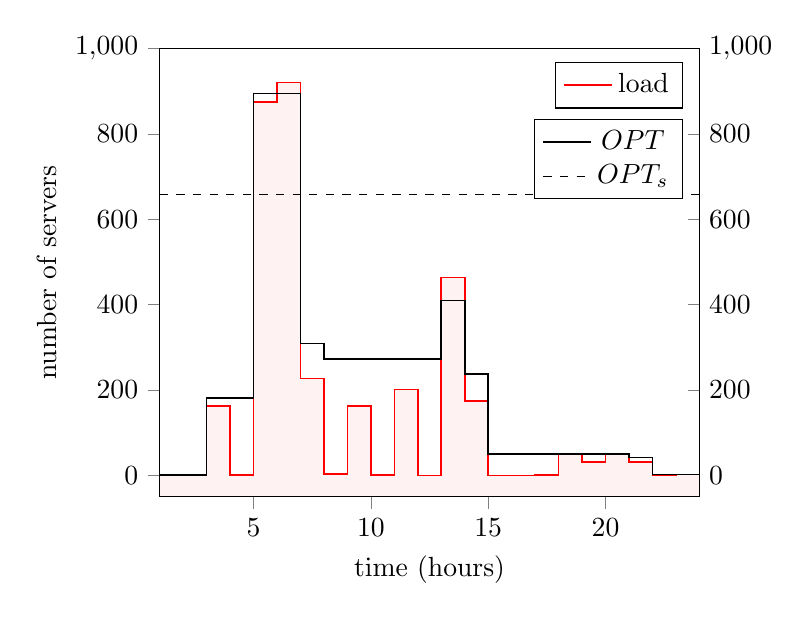
\begin{tikzpicture}

\begin{axis}[
legend pos=north east,
axis y line*=right,
axis x line=none,
xmin=1, xmax=24,
ymin=-50, ymax=1000,
% ylabel=load
]
\addplot [semithick, red, const plot mark left, name path=A]
table {%
1 1
2 0
3 163
4 1
5 874
6 920
7 227
8 3
9 162
10 1
11 201
12 0
13 464
14 174
15 0
16 0
17 1
18 50
19 32
20 50
21 31
22 0
23 2
24 1
};
\addlegendentry{load}

\addplot+[draw=none,domain=0:24,name path=B] {-10000};
\addplot+[red!5] fill between[of=A and B];
\end{axis}

\begin{axis}[
legend style={at={(axis cs:23.3,835)},anchor=north east},
tick align=outside,
tick pos=left,
% x grid style={white!69.0196078431373!black},
xlabel={time (hours)},
xmin=1, xmax=24,
% xtick style={color=black},
% y grid style={white!69.0196078431373!black},
ylabel={number of servers},
ymin=-50, ymax=1000,
% ytick style={color=black}
]
\addplot [semithick, black, const plot mark left]
table {%
1 1
2 1
3 181
4 181
5 895
6 895
7 309
8 273
9 273
10 273
11 273
12 273
13 410
14 237
15 50
16 50
17 50
18 50
19 50
20 50
21 42
22 2
23 2
24 1
};
\addlegendentry{$OPT$}

\draw[dashed, color=black] (axis cs:\pgfkeysvalueof{/pgfplots/xmin},659) -- (axis cs:\pgfkeysvalueof{/pgfplots/xmax},659);
\addlegendimage{dashed, color=black}
\addlegendentry{$OPT_s$}
\end{axis}

\end{tikzpicture}
}
    \caption{LANL Mustang}
    \end{subfigure}
    \begin{subfigure}[b]{.35\linewidth}
    \resizebox{\textwidth}{!}{% This file was created by tikzplotlib v0.9.9.
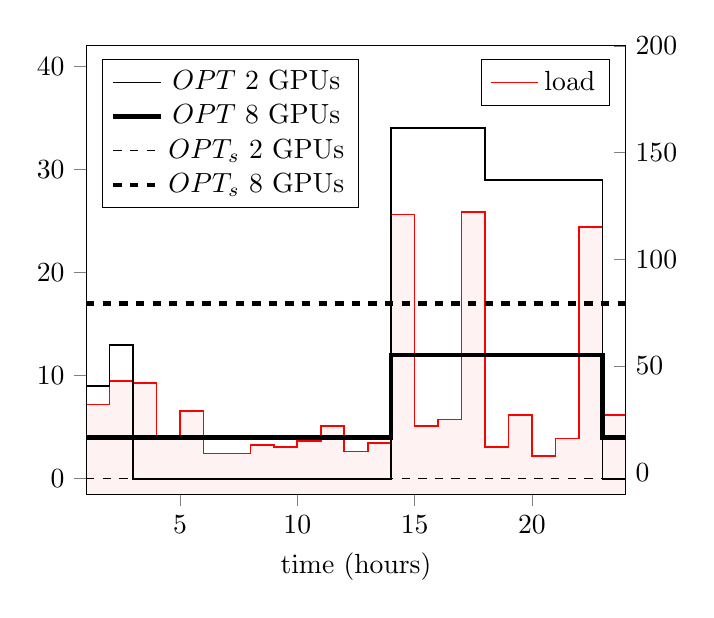
\begin{tikzpicture}

\begin{axis}[
legend pos=north east,
axis y line*=right,
axis x line=none,
xmin=1, xmax=24,
ymin=-10, ymax=200,
% ylabel=load
]
\addplot [semithick, red, const plot mark left, name path=A]
table {%
1 32
2 43
3 42
4 16
5 29
6 9
7 9
8 13
9 12
10 15
11 22
12 10
13 14
14 121
15 22
16 25
17 122
18 12
19 27
20 8
21 16
22 115
23 27
24 23
};
\addlegendentry{load}

\addplot+[draw=none,domain=0:24,name path=B] {-10000};
\addplot+[red!5] fill between[of=A and B];
\end{axis}

\begin{axis}[
legend pos=north west,
tick align=outside,
tick pos=left,
% x grid style={white!69.0196078431373!black},
xlabel={time (hours)},
xmin=1, xmax=24,
% xtick style={color=black},
% y grid style={white!69.0196078431373!black},
% ylabel={number of servers},
ymin=-1.5, ymax=42,
% ytick style={color=black}
]
\addplot [semithick, black, const plot mark left]
table {%
1 9
2 13
3 0
4 0
5 0
6 0
7 0
8 0
9 0
10 0
11 0
12 0
13 0
14 34
15 34
16 34
17 34
18 29
19 29
20 29
21 29
22 29
23 0
24 0
};
\addlegendentry{$OPT$ 2 GPUs}
\addplot [ultra thick, black, const plot mark left]
table {%
1 4
2 4
3 4
4 4
5 4
6 4
7 4
8 4
9 4
10 4
11 4
12 4
13 4
14 12
15 12
16 12
17 12
18 12
19 12
20 12
21 12
22 12
23 4
24 4
};
\addlegendentry{$OPT$ 8 GPUs}

\draw[dashed, color=black] (axis cs:\pgfkeysvalueof{/pgfplots/xmin},0) -- (axis cs:\pgfkeysvalueof{/pgfplots/xmax},0);
\addlegendimage{dashed, color=black}
\addlegendentry{$OPT_s$ 2 GPUs}
\draw[dashed, ultra thick, color=black] (axis cs:\pgfkeysvalueof{/pgfplots/xmin},17) -- (axis cs:\pgfkeysvalueof{/pgfplots/xmax},17);
\addlegendimage{dashed, ultra thick, color=black}
\addlegendentry{$OPT_s$ 8 GPUs}
\end{axis}

\end{tikzpicture}
}
    \caption{Microsoft Fiddle}
    \end{subfigure}
    \par\bigskip
    \begin{subfigure}[b]{.38\linewidth}
    \resizebox{\textwidth}{!}{% This file was created by tikzplotlib v0.9.9.
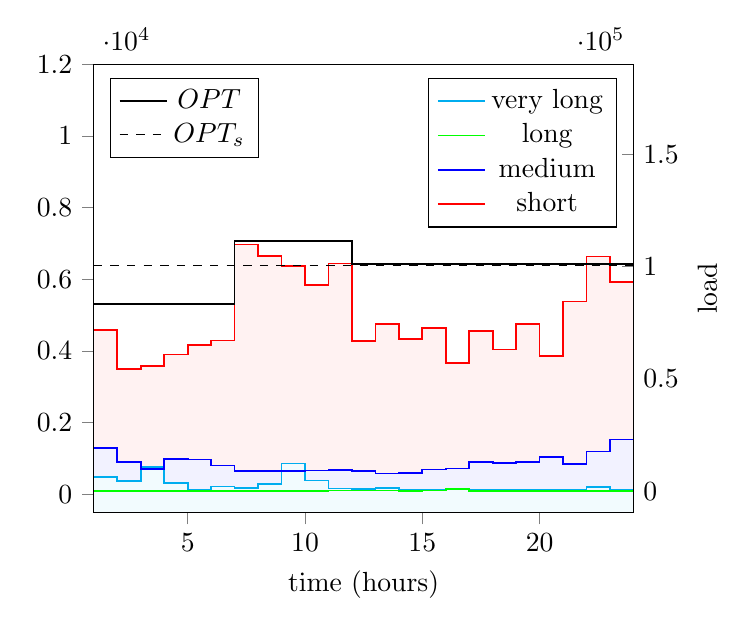
\begin{tikzpicture}

\begin{axis}[
legend pos=north east,
% stack plots=y,
axis y line*=right,
axis x line=none,
xmin=1, xmax=24,
ymin=-9500, ymax=190000,
ylabel=load
]
\addplot [semithick, cyan, const plot mark left,name path=A4]
table {%
1 6388
2 4608
3 10887
4 3643
5 719
6 2126
7 1409
8 3239
9 12372
10 4711
11 1252
12 1090
13 1508
14 815
15 612
16 1032
17 431
18 488
19 402
20 603
21 790
22 1806
23 606
24 5420
};
\addlegendentry{very long}
\addplot [semithick, green, const plot mark left,name path=A3]
table {%
1 154
2 58
3 35
4 58
5 53
6 23
7 56
8 88
9 106
10 127
11 371
12 350
13 238
14 209
15 313
16 865
17 128
18 152
19 124
20 138
21 123
22 88
23 37
24 71
};
\addlegendentry{long}
\addplot [semithick, blue, const plot mark left,name path=A2]
table {%
1 19071
2 12928
3 9869
4 14223
5 14023
6 11464
7 9042
8 9103
9 9109
10 9150
11 9320
12 9014
13 7913
14 8132
15 9713
16 10031
17 12864
18 12558
19 12909
20 15273
21 11957
22 17614
23 23001
24 16746
};
\addlegendentry{medium}
\addplot [semithick, red, const plot mark left,name path=A1]
table {%
1 71738
2 54322
3 55729
4 60749
5 64916
6 67104
7 109698
8 104588
9 100065
10 91810
11 101320
12 66868
13 74260
14 67624
15 72631
16 57123
17 71217
18 63062
19 74424
20 60045
21 84472
22 104435
23 93108
24 87287
};
\addlegendentry{short}

\addplot+[draw=none,domain=0:24,name path=B] {-10000};
\addplot+[red!5] fill between[of=A1 and B];
\addplot+[blue!5] fill between[of=A2 and B];
\addplot+[green!5] fill between[of=A3 and B];
\addplot+[cyan!5] fill between[of=A4 and B];
\end{axis}

\begin{axis}[
legend pos=north west,
tick align=outside,
tick pos=left,
% x grid style={white!69.0196078431373!black},
xlabel={time (hours)},
xmin=1, xmax=24,
% xtick style={color=black},
% y grid style={white!69.0196078431373!black},
% ylabel={proportion of iterations},
ymin=-510, ymax=12000,
% ytick style={color=black}
]
\addplot [semithick, black, const plot mark left]
table {%
1 5313
2 5313
3 5313
4 5313
5 5313
6 5313
7 7071
8 7071
9 7071
10 7071
11 7071
12 6428
13 6428
14 6428
15 6428
16 6428
17 6428
18 6428
19 6428
20 6428
21 6428
22 6428
23 6428
24 6428
};
\addlegendentry{$OPT$}

\draw[dashed, color=black] (axis cs:\pgfkeysvalueof{/pgfplots/xmin},6383) -- (axis cs:\pgfkeysvalueof{/pgfplots/xmax},6383);
\addlegendimage{dashed, color=black}
\addlegendentry{$OPT_s$}
\end{axis}

\end{tikzpicture}
}
    \caption{Alibaba}
    \end{subfigure}
\end{figure}
\end{frame}

\begin{frame}{Performance metrics}
\begin{itemize}
    \item \b{normalized cost}: $c(ALG) / c(OPT)$\pause
    \item \b{cost reduction}: \begin{align*}
        \frac{c(OPT_s) - c(ALG)}{c(OPT_s)}
    \end{align*}\pause
    \item \b{static/dynamic ratio}: $c(OPT_s) / c(OPT)$
\end{itemize}
\end{frame}

\begin{frame}{Results in one dimension}
\begin{figure}
    \begin{subfigure}[b]{.50\linewidth}
    \resizebox{\textwidth}{!}{% This file was created by tikzplotlib v0.9.9.
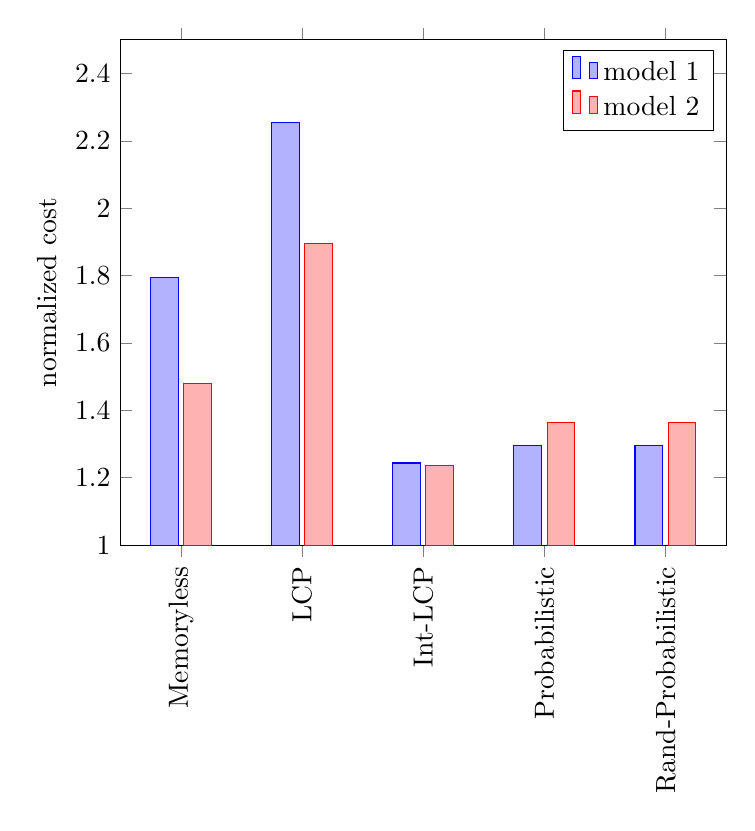
\begin{tikzpicture}

\begin{axis}[
ybar,
% bar width=0.5cm,
height=8cm,
% tick align=outside,
% tick pos=left,
% x grid style={white!69.0196078431373!black},
% xlabel={$OPT_s / OPT$},
xmin=-0.5, xmax=4.5,
xtick={0,1,2,3,4,5,6},
xticklabel style={rotate=90.0},
xticklabels={Memoryless,LCP,Int-LCP,Probabilistic,Rand-Probabilistic},
% xtick style={color=black},
% y grid style={white!69.0196078431373!black},
ylabel={normalized cost},
ymin=1, ymax=2.5,
% /pgf/number format/precision=5,
% ytick style={color=black}
]
\addplot
table {%
0 1.793108632
1 2.254697647
2 1.243801312
3 1.296624346
4 1.294611567
};
\addplot
table {%
0 1.479166878
1 1.895323607
2 1.235296539
3 1.363824754
4 1.363368466
};
\legend{model 1, model 2}
\end{axis}

\end{tikzpicture}
}
    \caption{LANL Mustang}
    \end{subfigure}
    \begin{subfigure}[b]{.48\linewidth}
    \resizebox{\textwidth}{!}{% This file was created by tikzplotlib v0.9.9.
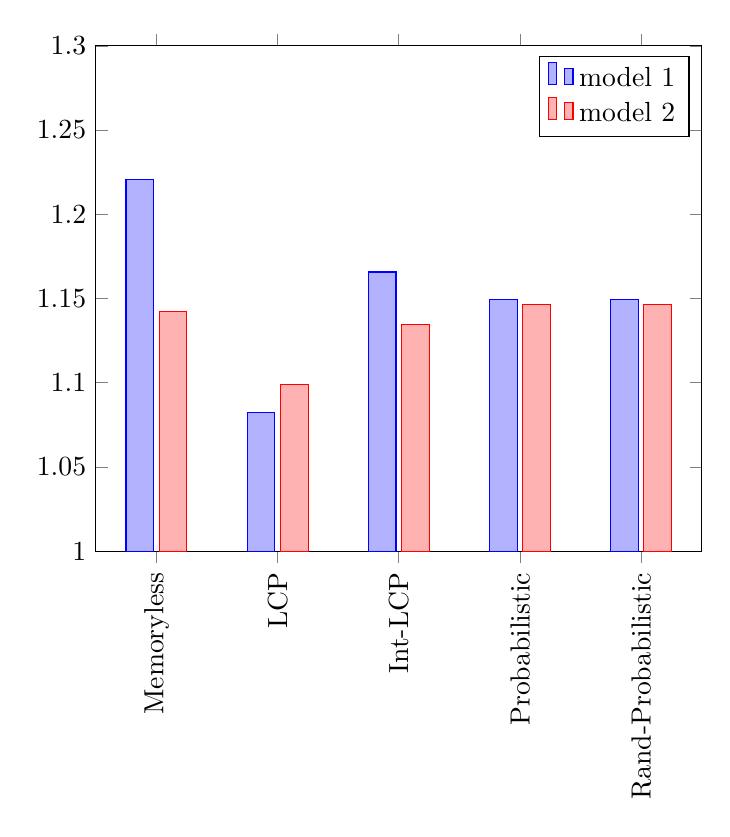
\begin{tikzpicture}

\begin{axis}[
ybar,
% bar width=0.5cm,
height=8cm,
% tick align=outside,
% tick pos=left,
% x grid style={white!69.0196078431373!black},
% xlabel={$OPT_s / OPT$},
xmin=-0.5, xmax=4.5,
xtick={0,1,2,3,4,5,6},
xticklabel style={rotate=90.0},
xticklabels={Memoryless,LCP,Int-LCP,Probabilistic,Rand-Probabilistic},
% xtick style={color=black},
% y grid style={white!69.0196078431373!black},
% ylabel={normalized cost},
ymin=1, ymax=1.3,
% /pgf/number format/precision=5,
% ytick style={color=black}
]
\addplot
table {%
0 1.220650656
1 1.082388905
2 1.165761722
3 1.149285464
4 1.149467892
};
\addplot
table {%
0 1.142369131
1 1.098736948
2 1.134416689
3 1.146620801
4 1.146662935
};
\legend{model 1, model 2}
\end{axis}

\end{tikzpicture}
}
    \caption{Alibaba}
    \end{subfigure}
\end{figure}
\end{frame}

\begin{frame}{Results in one dimension}
\begin{figure}
    \begin{subfigure}[b]{.38\linewidth}
    \resizebox{\textwidth}{!}{\pgfplotstableread{
X Y
2.115 1.1862049328218298
1.913 1.1540470009508415
1.549 1.0479312893570394
6.575 2.4294509720294735
3.822 1.9696643
1.339 1.068293057
}\a
\pgfplotstableread{
X Y
2.115 1.071842679781245
1.913 1.0433664197908732
1.549 1
6.575 1.9200838991565596
3.822 1.29969
1.339 1.011010843
}\b

\begin{tikzpicture}
\begin{axis}[
legend pos=south east,
ylabel={static/dynamic ratio},
xlabel={PMR}]
\addplot [only marks, blue, mark = o] table {\a};
\addlegendentry{model 1}
\addplot [only marks, red, mark = o] table {\b};
\addlegendentry{model 2}
\addplot [thick, blue] table[
    y={create col/linear regression={y=Y}}
] % compute a linear regression from the input table
{\a};
\addplot [thick, red] table[
    y={create col/linear regression={y=Y}}
] % compute a linear regression from the input table
{\b};
\end{axis}
\end{tikzpicture}}
    \end{subfigure}\pause
    \begin{subfigure}[b]{.38\linewidth}
    \resizebox{\textwidth}{!}{\pgfplotstableread{
X Y
1.1862049328218298 1.217963395
1.1862049328218298 1.073752054
1.1862049328218298 1.203176915
1.1862049328218298 1.213633822
1.1862049328218298 1.215964525
1.1540470009508415 1.264233547
1.1540470009508415 1.126679608
1.1540470009508415 1.177011887
1.1540470009508415 1.215947005
1.1540470009508415 1.215947005
1.0479312893570394 1.267149747
1.0479312893570394 1.144691647
1.0479312893570394 1.241611332
1.0479312893570394 1.246984786
1.0479312893570394 1.24775128
2.4294509720294735 1.793108632
2.4294509720294735 2.254697647
2.4294509720294735 1.243801312
2.4294509720294735 1.296624346
2.4294509720294735 1.294611567
1.068293057 1.220650656
1.068293057 1.082388905
1.068293057 1.165761722
1.068293057 1.149285464
1.068293057 1.149467892
}\a
\pgfplotstableread{
X Y
1.071842679781245 1.157784554
1.071842679781245 1.088245181
1.071842679781245 1.214821767
1.071842679781245 1.212900741
1.071842679781245 1.213648703
1.0433664197908732 1.205891207
1.0433664197908732 1.166348954
1.0433664197908732 1.153605888
1.0433664197908732 1.221498393
1.0433664197908732 1.222450113
1 1.042592762
1 1.002849673
1 1.07620715
1.9200838991565596 1.479166878
1.9200838991565596 1.895323607
1.9200838991565596 1.235296539
1.9200838991565596 1.363824754
1.9200838991565596 1.363368466
1.011010843 1.142369131
1.011010843 1.098736948
1.011010843 1.134416689
1.011010843 1.146620801
1.011010843 1.146662935
}\b

\begin{tikzpicture}
\begin{axis}[
legend pos=north west,
xlabel={static/dynamic ratio},
ylabel={normalized cost}]
\addplot [only marks, blue, mark = o] table {\a};
\addlegendentry{model 1}
\addplot [only marks, red, mark = o] table {\b};
\addlegendentry{model 2}
\addplot [thick, blue] table[
    y={create col/linear regression={y=Y}}
] % compute a linear regression from the input table
{\a};
\addplot [thick, red] table[
    y={create col/linear regression={y=Y}}
] % compute a linear regression from the input table
{\b};
\end{axis}
\end{tikzpicture}}
    \end{subfigure}\pause
    \par\bigskip
    \begin{subfigure}[b]{.38\linewidth}
    \resizebox{\textwidth}{!}{\pgfplotstableread{
X Y
-2.6773166 1.217963395
9.4800549 1.073752054
-1.43078 1.203176915
-2.3123229 1.213633822
-2.508807 1.215964525
-9.5478387 1.264233547
2.3714279 1.126679608
-1.9899437 1.177011887
-5.3637334 1.215947005
-5.3637334 1.215947005
-20.9191633 1.267149747
-9.233464 1.144691647
-18.4821319 1.241611332
-18.9948996 1.246984786
-19.0680432 1.24775128
26.1928455 1.793108632
7.1931201 2.254697647
48.8031935 1.243801312
46.6289149 1.296624346
46.711764 1.294611567
-14.2617794 1.220650656
-1.3194739 1.082388905
-09.1237759 1.165761722
-07.5814783 1.149285464
-07.5985549 1.149467892
}\a
\pgfplotstableread{
X Y
-8.0181426 1.157784554
-1.5303087 1.088245181
-13.3395591 1.214821767
-13.1603326 1.212900741
-13.2301154 1.213648703
-15.5769616 1.205891207
-11.7870895 1.166348954
-10.5657481 1.153605888
-17.0728106 1.221498393
-17.1640269 1.222450113
-4.2592762 1.042592762
-0.2849673 1.002849673
-7.620715 1.07620715
22.9634247 1.479166878
1.2895422 1.895323607
35.6644499 1.235296539
28.9705645 1.363824754
28.9943285 1.363368466
-12.9927675 1.142369131
-8.6770686 1.098736948
-12.2061842 1.134416689
-13.413304 1.146620801
-13.4174715 1.146662935
}\b

\begin{tikzpicture}
\begin{axis}[
legend pos=north east,
xlabel={cost reduction (\%)},
ylabel={normalized cost}]
\addplot [only marks, blue, mark = o] table {\a};
\addlegendentry{model 1}
\addplot [only marks, red, mark = o] table {\b};
\addlegendentry{model 2}
\addplot [thick, blue] table[
    y={create col/linear regression={y=Y}}
] % compute a linear regression from the input table
{\a};
\addplot [thick, red] table[
    y={create col/linear regression={y=Y}}
] % compute a linear regression from the input table
{\b};
\end{axis}
\end{tikzpicture}}
    \end{subfigure}
\end{figure}
\end{frame}

\begin{frame}{Overview of results in multiple dimensions}
\begin{itemize}
    \item lazy budgeting algorithms perform nearly optimally (normalized cost $\in [1.05, 1.25]$), without consideration of revenue loss\pause
    \item descent methods achieve normalized costs of $\approx 2.5$, assuming the decision space is Euclidean
\end{itemize}
\end{frame}

\begin{frame}{Results with predictions}
\begin{figure}
    \begin{subfigure}[b]{.51\linewidth}
    \resizebox{\textwidth}{!}{% This file was created by tikzplotlib v0.9.9.
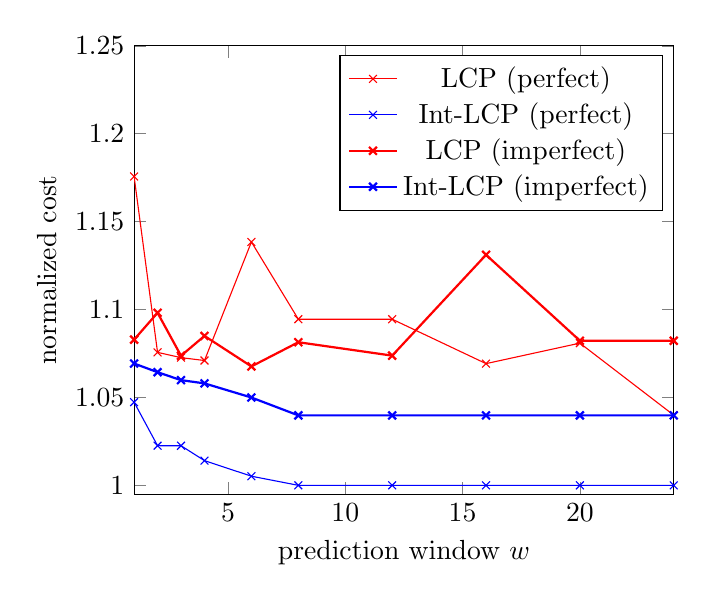
\begin{tikzpicture}

\begin{axis}[
% tick align=outside,
% tick pos=left,
% x grid style={white!69.0196078431373!black},
xlabel={prediction window $w$},
xmin=1, xmax=24,
% xtick style={color=black},
% y grid style={white!69.0196078431373!black},
ylabel={normalized cost},
ymin=0.995, ymax=1.25,
% ytick style={color=black}
]
\addplot [mark=x,red]
table {%
0 1.098736948
1 1.175687427
2 1.075631818
3 1.072634645
4 1.070999275
6 1.138422029
8 1.094499546
12 1.094499546
16 1.06923045
20 1.080885023
24 1.039921325
};
\addlegendentry{LCP (perfect)}
\addplot [mark=x,blue]
table {%
0 1.134416689
1 1.047299695
2 1.022549638
3 1.022528928
4 1.014063942
6 1.00519416
8 1
12 1
16 1
20 1
24 1
};
\addlegendentry{Int-LCP (perfect)}
\addplot [mark=x,red,thick]
table {%
0 1.098736948
1 1.082887541
2 1.098133413
3 1.073693844
4 1.08498568
6 1.067637295
8 1.081397557
12 1.073772973
16 1.13110595
20 1.08225852
24 1.08225852
};
\addlegendentry{LCP (imperfect)}
\addplot [mark=x,blue,thick]
table {%
0 1.134416689
1 1.069284948
2 1.064359748
3 1.059832012
4 1.057992166
6 1.049956689
8 1.039784723
12 1.039784723
16 1.039784723
20 1.039784723
24 1.039784723
};
\addlegendentry{Int-LCP (imperfect)}
\end{axis}

\end{tikzpicture}
}
    \caption{LCP and Int-LCP}
    \end{subfigure}\pause
    \begin{subfigure}[b]{.48\linewidth}
    \resizebox{\textwidth}{!}{% This file was created by tikzplotlib v0.9.9.
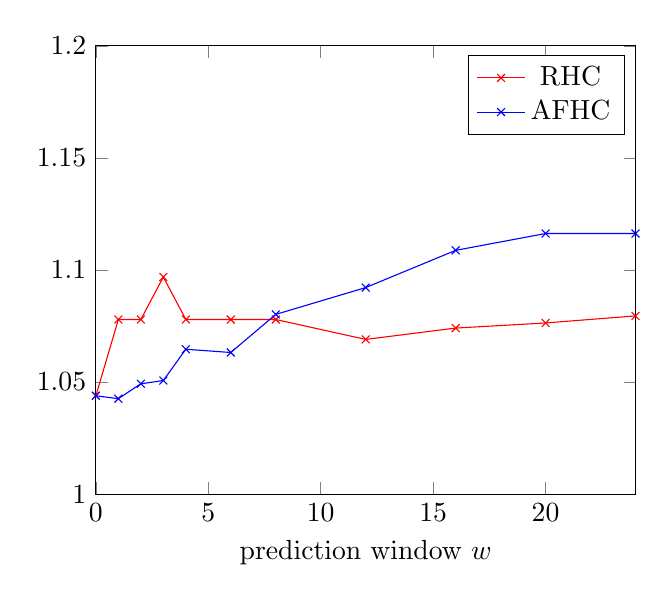
\begin{tikzpicture}

\begin{axis}[
% tick align=outside,
% tick pos=left,
% x grid style={white!69.0196078431373!black},
xlabel={prediction window $w$},
xmin=0, xmax=24,
% xtick style={color=black},
% y grid style={white!69.0196078431373!black},
% ylabel={normalized cost},
ymin=1, ymax=1.2,
% ytick style={color=black}
]
\addplot [mark=x,red]
table {%
0 1.043876404
1 1.077904071
2 1.077904071
3 1.096849433
4 1.077911928
6 1.077904071
8 1.077904071
12 1.06902603
16 1.0740756
20 1.076362197
24 1.079518259
};
\addlegendentry{RHC}
\addplot [mark=x,blue]
table {%
0 1.043876404
1 1.042590748
2 1.049217045
3 1.050676806
4 1.064636454
6 1.063182574
8 1.080176738
12 1.092145632
16 1.108752789
20 1.116262537
24 1.116262537
};
\addlegendentry{AFHC}
\end{axis}

\end{tikzpicture}
}
    \caption{RHC and AFHC}
    \end{subfigure}
\end{figure}
\end{frame}

\section{Future work}

\begin{frame}{Future work}
\begin{itemize}
    \item compare performance to algorithms for convex body chasing\pause
    \item performance of algorithms in other applications\pause
    \item appropriate modeling of long-running jobs\pause
    \item SOCO without lookahead\pause
    \item better algorithms to make use of predictions
\end{itemize}
\end{frame}

\begin{frame}
\centering \large
Thanks for your attention!
Questions?
\end{frame}

% \begin{frame}[allowframebreaks]
% \printbibliography
% \end{frame}

\end{document}
